\section{Superposition of Waves}

When two of more waves meet together, the resultant motion is a combination of the individuals. They can form a \emph{resultant wave} when they overlap, after which they cross one another and neither is affected. In this chapter, we will study the principle of superposition, and look at two important consequences: the phenomenon of \emph{interference} and \emph{stationary waves}.

\subsection{superposition of waves}



\subsection{principle of superposition}

\begin{ilight}
	 when two (or more) waves meet to form a resultant wave, the \keypoint{principle of superposition} states that the resultant displacement is the vector sum of each individual displacement\index{superposition of waves!principle of superposition}
\end{ilight}

\example{Displacement–time graphs for two waves $A$ and $B$ meeting at some point, together with the resultant wave formed at that point.}

\begin{figure}[ht]
	\centering
	\begin{minipage}{0.45\textwidth}
		\centering
		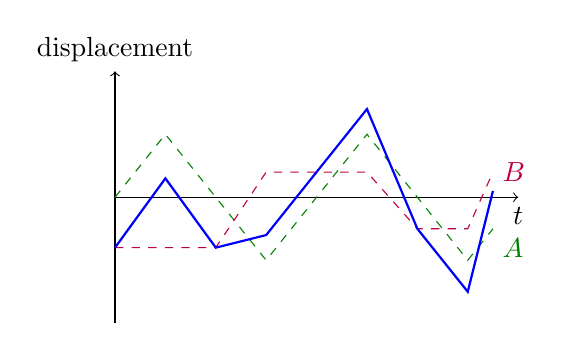
\begin{tikzpicture}[scale=0.8]
		\draw [->] (0,-2) -- (0,2) node[above]{displacement};
		\draw [->] (0,0) -- (6.4,0) node[below]{$t$};
		\draw [Green, dashed] (0,0) --++ (0.8,1) --++ (1.6, -2) --++ (1.6,2) --++ (1.6, -2) --++ (0.4,0.5) node[below right]{$A$};
		\draw [purple, dashed] (0,-0.8) -- (1.6,-0.8) -- (2.4, 0.4) -- (4 ,0.4) -- (4.8, -0.5) -- (5.6, -0.5) -- (6, 0.4) node[right]{$B$}; 
		\draw [thick, blue] (0,-0.8) -- (0.8, 0.3) -- (1.6, -0.8) -- (2.4, -0.6) -- (4, 1.4) -- (4.8, -0.5) -- (5.6, -1.5) -- (6,0.1);
		\end{tikzpicture}
	\end{minipage}\hfil
	\begin{minipage}{0.45\textwidth}
		\centering
		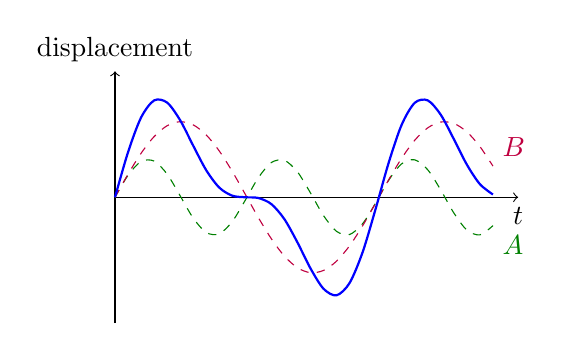
\begin{tikzpicture}[scale=0.8]
		\draw [->] (0,-2) -- (0,2) node[above]{displacement};
		\draw [->] (0,0) -- (6.4,0) node[below]{$t$};
		\draw [Green,dashed,domain=0:6,samples=30,smooth] plot (\x,{0.6*sin(\x*3 r)}) node[below right]{$A$};
		\draw [purple,dashed,domain=0:6,samples=30,smooth] plot (\x,{1.2*sin(\x*1.5 r)}) node[above right]{$B$};
		\draw [thick,blue,domain=0:6,samples=30,smooth] plot (\x,{1.2*sin(\x*1.5 r) + 0.6*sin(\x*3 r)});
		\end{tikzpicture}
	\end{minipage}
\end{figure}

\cmt two important situations are constructive superposition and destructive superposition\index{superposition of waves!constructive superposition}\index{superposition of waves!destructive superposition}

\cmt \keypoint{constructive superposition} occurs when resultant wave has greatest possible amplitude
	
	this happens when peaks of the two waves meet together (also trough meets trough)\footnote{This statement is implicitly for transverse waves. For longitudinal waves to superpose constructively, the regions of compression (or rarefaction) must overlap.}
	
	peaks of both waves must arrive with a time difference $\Delta t = 0, \, T, \, 2T, \cdots$
	
\cmt \keypoint{destructive superposition} occurs when amplitudes of each wave cancel out one another
	
	this happens when peak of one wave overlaps with trough of the other wave
	
	peaks of both waves must arrive with a time difference $\Delta t = \frac{1}{2}T, \, \frac{3}{2}T, \, \frac{5}{2}T, \cdots$

\begin{figure}[ht]
	\centering
	\noindent\begin{minipage}{0.45\linewidth}
		\centering
		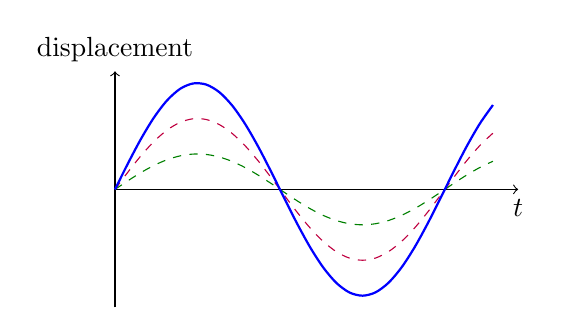
\begin{tikzpicture}[xscale=0.8, yscale=0.75]
		\draw [->] (0,-2) -- (0,2) node[above]{displacement};
		\draw [->] (0,0) -- (6.4,0) node[below]{$t$};
		\draw [Green, dashed,domain=0:6,samples=30,smooth] plot (\x,{0.6*sin(\x*1.2 r)});
		\draw [purple, dashed,domain=0:6,samples=30,smooth] plot (\x,{1.2*sin(\x*1.2 r)});
		\draw [thick,blue,domain=0:6,samples=30,smooth,variable=\x] plot (\x,{1.8*sin(\x*1.2 r)});
		\end{tikzpicture}
	\end{minipage}\hfil
	\begin{minipage}{0.45\linewidth}
		\centering
		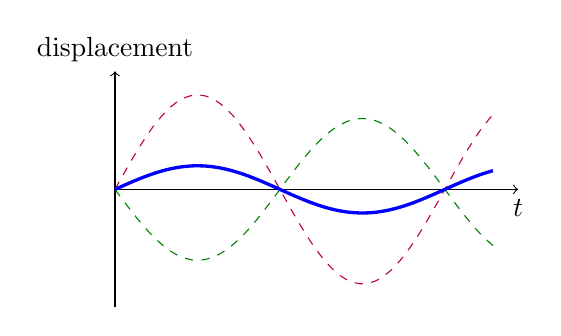
\begin{tikzpicture}[xscale=0.8, yscale=0.75]
		\draw [->] (0,-2) -- (0,2) node[above]{displacement};
		\draw [->] (0,0) -- (6.4,0) node[below]{$t$};
		\draw [Green,dashed,domain=0:6,samples=30,smooth] plot (\x,{-1.2*sin(\x*1.2 r)});
		\draw [purple ,dashed,domain=0:6,samples=30,smooth] plot (\x,{1.6*sin(\x*1.2 r)});
		\draw [very thick,blue,domain=0:6,samples=30,smooth] plot (\x,{0.4*sin(\x*1.2 r)});
		\end{tikzpicture}
	\end{minipage}\hfil
	\caption{constructive and destructive superposition of two transvers waves}
\end{figure}

\begin{figure}[htp]
	\centering
	\noindent\begin{minipage}{0.5\linewidth}
		\centering
		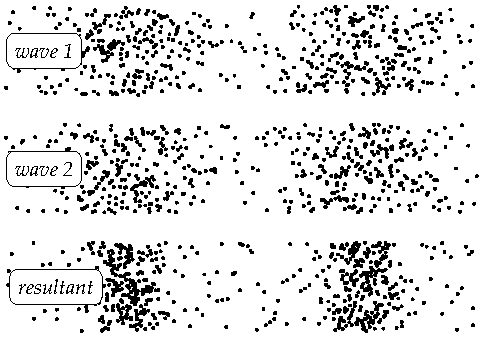
\includegraphics[width=.95\textwidth]{longitudinal+I.pdf}
	\end{minipage}\hfil
	\begin{minipage}{0.5\linewidth}
		\centering
		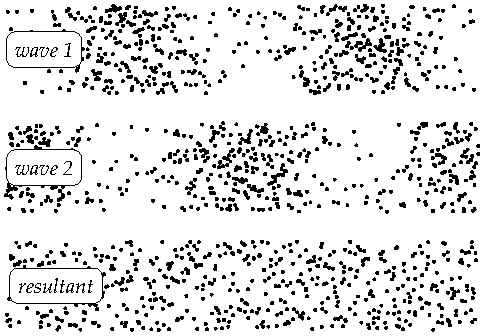
\includegraphics[width=.95\textwidth]{longitudinal-I.pdf}
	\end{minipage}
	\caption*{constructive and destructive superposition of two sound waves} 
\end{figure}



\subsection{path difference}

one way to compare how much peaks of two waves differ is using the \keypoint{path difference}\index{path difference}

when two waves meet at a point, each wave travels a distance from its source

the difference between distances travelled by the two waves is the path difference $\Delta L$

\cmt we can tell whether two waves superpose constructively or destructively by path difference

{

\centering
\vspace*{6pt}
\begin{tcolorbox}[colframe=orange, colback=yellow!30, width=0.65\textwidth]
	\setlength{\baselineskip}{\baselineskip}%
	
	\centering
	
	if ${\Delta L = 0, \, \lambda, \, 2\lambda, \cdots}$, then superposition is constructive
	
	if ${\Delta L = \frac{\lambda}{2}, \, \frac{3\lambda}{2}, \, \frac{5\lambda}{2}, \cdots}$, then superposition is destructive
	
\end{tcolorbox}\vspace*{-4pt}

}

\newpage

\example{Two loudspeakers are wired to produce identical sound signals in unison. The sound wave produced has a wavelength of 80 cm. Describe the volume you hear when you are at a distance of (a) 10 m from both speakers, (b) 10 m from one speaker and 12 m from the other?}

\begin{soln} path difference for case (a): $\Delta L = 10 - 10  = 0$

so constructive superposition, resultant amplitude is large, a loud sound is heard

path difference for case (b): $\Delta L = 12 - 10 = 2.0 \text{ m} \RA \Delta L = \frac{5}{2}\lambda$

so destructive superposition, resultant amplitude is small, sound is quiet \end{soln}

\subsection{phase difference}

when two waves or two vibrating particles are compared, it is also useful to describe how much one is out of step with the other in terms of their \keypoint{phase difference}\index{phase difference} ($\Delta \phi$)
\footnote{More logically, we should first define the notion of \emph{phase angle} before talking about the \emph{phase difference}, which is simply the difference between the phase angles of two waves.
	
	Wave motion can generally be described by sine (or cosine) functions. Since the initial displacement of a wave is not necessarily zero, one can introduce a constant term that appears in the argument of the sine function. This term shifts the origin of the sine, and we call that the \emph{phase angle} $\phi$ of the wave, measured in radians (or degrees). One can think of $\phi$ as a number giving the fraction in a complete oscillation.
	
	In particular, the displacement $y$ of a transverse wave along the direction $x$ of energy transfer can be given by: $y = A \sin\left( \frac{2\pi x}{\lambda} - \frac{2\pi t}{T} + \phi \right)$. You can verify that this indeed describes a sinusoidal wave of wavelength $\lambda$ and period $T$ travelling at speed $v = \frac{\lambda}{T}$, while $\phi$ determines when and where the peaks show up.}

\cmt phase difference is measured in radians (rad) or degrees ($^\circ$)

\cmt if two waves have a phase difference $\Delta \phi = 0,2\pi,4\pi,\cdots$, the two waves are said to be \keypoint{in phase}\footnote{If $\Delta \phi$ is given in degrees, then two waves are in phase if $\Delta \phi = 0, \, 360^\circ, \, 720^\circ, \cdots$}

in this case, peak of one wave overlaps with peak of the other

\cmt if two waves are not in phase, then they are said to be \keypoint{out of phase}

\cmt if $\Delta \phi = \pi, 3\pi, 5\pi, \cdots$, then two waves are completely out of phase, or \keypoint{anti-phase}\footnote{If $\Delta \phi$ is given in degrees, then two waves are anti-phase if $\Delta \phi = 180^\circ, \, 540^\circ, \, 900^\circ, \cdots$}

in this case, peak of one wave meets the trough of the other


\cmt we can tell whether two waves superpose constructively or destructively by phase difference

{
	
	\centering
	\vspace*{6pt}
	\begin{tcolorbox}[colframe=orange, colback=yellow!30, width=0.65\textwidth]
		\setlength{\baselineskip}{\baselineskip}%
		
		\centering
		
		if ${\Delta \phi = 0, \, 2\pi, \,4\pi, \cdots}$, then superposition is constructive
		
		if ${\Delta \phi = \pi, \, 3\pi, \, 5\pi, \cdots}$, then superposition is destructive
		
	\end{tcolorbox}\vspace*{-4pt}
	
}






\newpage

\cmt phase difference can be related to path difference by: $ \boxed{ \frac{\Delta \phi}{2\pi} = \frac{\Delta L}{\lambda} = \frac{\Delta t}{T} } $

\example{The diagrams below each shows the displacement of a particular point in two transverse waves. If both waves are travelling in the same direction with a wavelength of 30 cm, what is the phase difference and path difference between each wave?}

\begin{figure}[htp]
	\centering
	\begin{minipage}{0.32\textwidth}
		\centering
		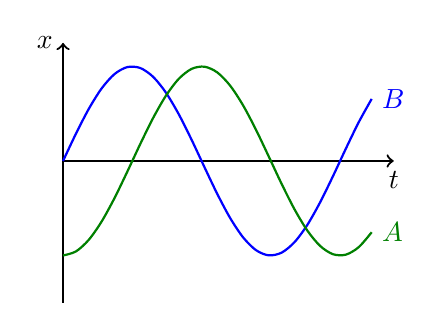
\begin{tikzpicture}[xscale=0.56,yscale=0.6]
		\draw [thick, ->] (0,0) --(7.5,0) node[below]{$t$};
		\draw [thick, ->] (0,-3) --(0,2.5) node[left]{$x$};
		\draw [thick,blue,domain=0:7,smooth] plot (\x,{2*sin(\x r)}) node[right]{$B$};
		\draw [thick,Green,domain=0:7,smooth] plot (\x,{2*sin(((\x - pi/2) r)}) node[right]{$A$};
		\end{tikzpicture}
		
		(a)
	\end{minipage}
	\begin{minipage}{0.32\textwidth}
		\centering
		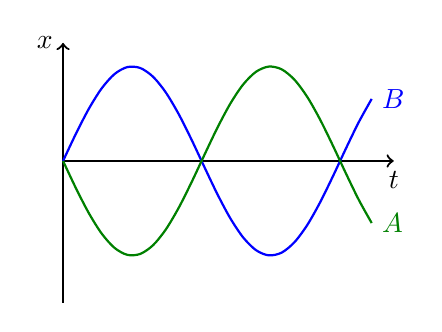
\begin{tikzpicture}[xscale=0.56,yscale=0.6]
		\draw [thick, ->] (0,0) --(7.5,0) node[below]{$t$};
		\draw [thick, ->] (0,-3) --(0,2.5) node[left]{$x$};
		\draw [thick,blue,domain=0:7,smooth] plot (\x,{2*sin(\x r)}) node[right]{$B$};
		\draw [thick,Green,domain=0:7,smooth] plot (\x,{2*sin(((\x - pi) r)}) node[right]{$A$};
		\end{tikzpicture}
		
		(b)
	\end{minipage}
	\begin{minipage}{0.32\textwidth}
		\centering
		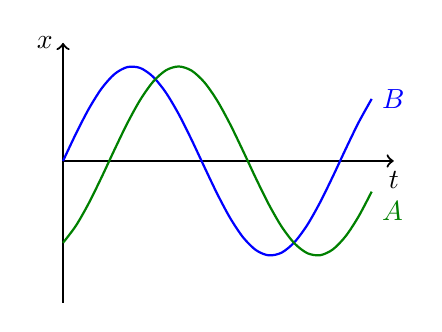
\begin{tikzpicture}[xscale=0.56,yscale=0.6]
		\draw [thick, ->] (0,0) --(7.5,0) node[below]{$t$};
		\draw [thick, ->] (0,-3) --(0,2.5) node[left]{$x$};
		\draw [thick,blue,domain=0:7,smooth] plot (\x,{2*sin(\x r)}) node[right]{$B$};
		\draw [thick,Green,domain=0:7,smooth] plot (\x,{2*sin(((\x - pi/3) r)}) node[below right]{$A$};
		\end{tikzpicture}
		
		(c)
	\end{minipage}
%	\caption*{examples of phases differences between two waves}
\end{figure}

\begin{soln}
(a) $\Delta t = \frac{1}{4}T \RA \Delta \phi = \frac{1}{4}\times 2\pi = \frac{1}{2}\pi, \quad \Delta L = \frac{1}{4} \lambda = \frac{1}{4}\times30 = 7.5 \text{ cm}$

\eqyskip (b) $\Delta t = \frac{1}{2}T \RA \Delta \phi = \frac{1}{2}\times 2\pi = \pi, \quad \Delta L = \frac{1}{2} \lambda = \frac{1}{2}\times30 = 15 \text{ cm}$

\eqyskip (c) $\Delta t = \frac{1}{6}T \RA \Delta \phi = \frac{1}{6}\times 2\pi = \frac{1}{3}\pi, \quad \Delta L = \frac{1}{6} \lambda = \frac{1}{6}\times30 = 5.0 \text{ cm}$ \end{soln}


\subsection*{brief summary}

conditions for constructive and destructive superposition can be summarised as follows:

\begin{center}
{\renewcommand{\arraystretch}{1.25}
\begin{tabular}{|c|c|c|}
	\hline
	& constructive superposition & destructive superposition \\
	\hline
	simple criteria & peak meets peak & peak meets trough \\
	\hline
	time difference & $\Delta t = n \cdot T$ & $\Delta t = \left(n+\frac{1}{2}\right) \cdot T$ \\
	\hline
	path difference & $\Delta L = n \cdot \lambda$ & $\Delta L = \left(n+\frac{1}{2}\right) \cdot \lambda$ \\
	\hline
	phase difference & $\Delta \phi = n\cdot 2\pi\,$ or $\,n\cdot 360^\circ$ & $\Delta \phi = \left(n+\frac{1}{2}\right)\cdot 2\pi \,$ or $\,\left(n+\frac{1}{2}\right)\cdot 360^\circ$ \\
	\hline
\end{tabular}
}
\end{center}

where $n$ is a whole number: $n=0, 1, 2, 3 \cdots$

remember that $\Delta t$, $\Delta L$ and $\Delta \phi$ are just different ways to describe how much one wave is ahead of/lag behind another wave, so they must be closely interrelated to each other






\subsection{interference}

\subsection{interference}

when two (or more) waves of constant phase difference meet, stable regions of constructive and destructive superposition are produced alternately, this phenomenon is called \keypoint{interference}\index{interference}



\begin{figure}[htp]
	\centering
	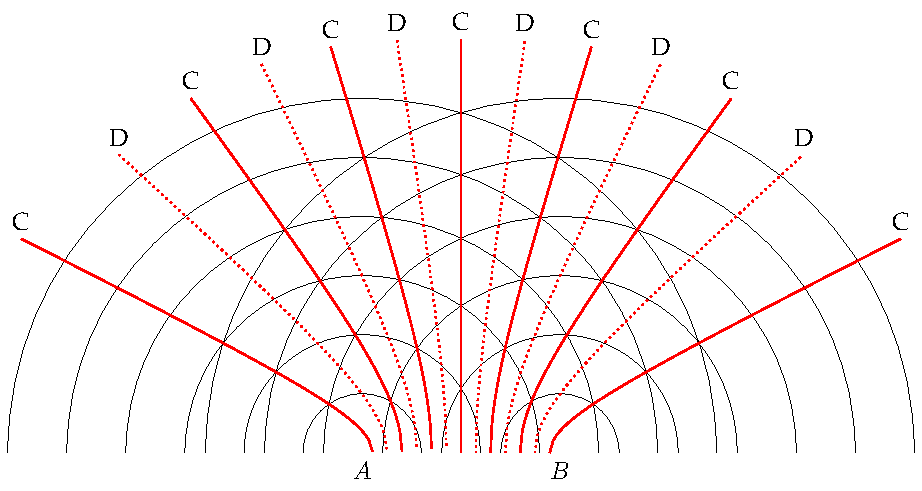
\includegraphics[width=1\textwidth]{interference.pdf}
	
	constructive (solid lines) and destructive (dashed lines) interference 
	
	of waves produced from two coherent sources $A$ and $B$
\end{figure}

\cmt regions of constructive interference are often called \emph{maxima}

\begin{compactitem}
	\item[--] points on line C$_0$ are of equal distance to wave sources, i.e., path difference $\Delta L = 0$
	
	so maxima are observed along C$_0$
	
	\item[--] points on C$_1$, C$_2$ and C$_3$ have path difference $\Delta L = \lambda, \, 2\lambda, \, 3\lambda$
	
	so maxima are also formed along C$_1$, C$_2$ and C$_3$
	
	\item[--] equivalently, points on C$_n$ have phase difference $\Delta \phi = n\cdot 2\pi$, where $n=0,1,2,3,\cdots$
\end{compactitem} 

\cmt regions of destructive interference are often called \emph{minima}

\begin{compactitem}
	\item[--] points on D$_1$, D$_2$ and D$_3$ have path difference $\Delta L = \frac{1}{2}\lambda, \, \frac{3}{2}\lambda, \, \frac{5}{2}\lambda$
	
	so maxima are also formed along D$_1$, D$_2$ and D$_3$
	
	\item[--] similarly, points on D$_n$ have phase difference $\Delta \phi = \left( n+\frac{1}{2} \right) \cdot 2\pi$, where $n=1,2,3,\cdots$
\end{compactitem} 






\newpage


\cmt stable interference means regions of maxima/minima remain maxima/minima

this requires \keypoint{coherent} wave sources, which means constant phase difference over time\index{coherence}

\cmt coherent waves usually come from same source, such as

\begin{compactitem}
	\item[--] dippers driven by a common vibrating beam in a ripple tank
	
	\item[--] loudspeakers driven by the same signal generator
\end{compactitem}

\begin{figure}[ht]
	\centering
	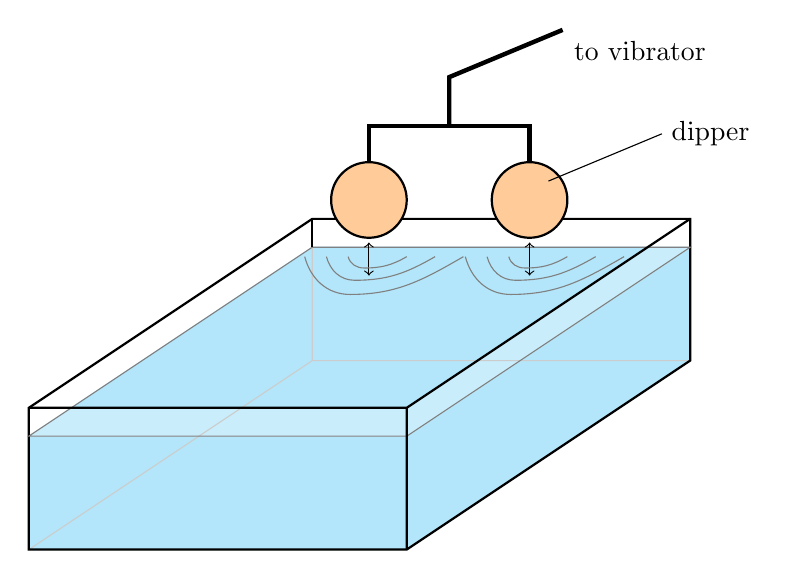
\begin{tikzpicture}[scale=1.2]
	% water in ripple tank
	\draw[cyan!30, fill] (2,-0.3) -- (2,-1.5) -- (-1,-3.5) -- (-5,-3.5) -- (-5,-2.3) -- (-2,-0.3) -- cycle;
	\draw[white, fill, opacity=0.3] (2,0) -- (2,-0.3) -- (-1,-2.3) -- (-5,-2.3) -- (-5,-2) -- (-1, -2) -- cycle;
	% outline for ripple tank
	\draw[gray!40] (-2,-0.3) -- (-2,-1.5) -- (2,-1.5) (-2,-1.5) -- (-5,-3.5);
	\draw[thick] (2,0) -- (2,-1.5) -- (-1,-3.5) -- (-5,-3.5) -- (-5,-2) -- (-2,0) -- cycle;
	\draw[thin, gray] (2,-0.3) -- (-1, -2.3) -- (-5, -2.3) -- (-2,-0.3) -- cycle;
	\draw[thick] (-5,-2) -- (-1, -2) -- (-1, -3.5) (-1, -2) -- (2,0);
	\draw[thick] (-2,0) -- (-2,-0.3);
	% dippers
	\foreach \x in {-0.8,0.9} {
		\draw[thick, fill=orange!40] ({-0.6+\x}, 0.2)  circle (0.4);
		\draw[ultra thick] ({-0.6+\x}, 0.6) -- ({-0.6+\x},1.0);
		\draw[<->] ({-0.6+\x}, -0.25) --++ (0,-0.35);
	}
	\draw[ultra thick] (-1.4, 0.98) -- (0.3, 0.98);
	\draw[ultra thick] (-0.55,1) --++ (0,0.5) --++ (1.2,0.5) node[below right]{to vibrator};
	\draw (0.5, 0.4) --++ (1.2,0.5) node[right]{dipper};
	% ripples
	\draw[gray] (-1.62,-0.4) [out=-75 , in=180] to (-1.45,-0.52) [out=0, in=210] to (-1.0,-0.4);
	\draw[gray] (-1.85,-0.4) [out=-75 , in=180] to (-1.55,-0.65) [out=0, in=210] to (-0.7,-0.4);
	\draw[gray] (-2.08,-0.4) [out=-75 , in=180] to (-1.6,-0.8) [out=0, in=210] to (-0.4,-0.4);
	\draw[gray] (0.08,-0.4) [out=-75 , in=180] to (0.25,-0.52) [out=0, in=210] to (0.7,-0.4);
	\draw[gray] (-0.15,-0.4) [out=-75 , in=180] to (0.15,-0.65) [out=0, in=210] to (1.0,-0.4);
	\draw[gray] (-0.38,-0.4) [out=-75 , in=180] to (0.1,-0.8) [out=0, in=210] to (1.3,-0.4);
	\end{tikzpicture}
	
	\caption*{demonstrating interferece of water waves in a ripple tank}
\end{figure}


\cmt interference are not observed for beams of light from different lamps or laser sources

this is because light from different sources are usually \emph{incoherent}\footnote{Emission of light is associated with the electronic transitions between energy levels in an atom, which is a completely random process. So in general separate light sources are not coherent.}

this can be overcome by dividing a single beam into several beams using a number of slits

common apparatuses of doing so are the \emph{double-slit} and \emph{diffraction gratings}

\example{Two coherent waves meet in space, one of which has an amplitude of 0.30 cm and the other of 0.20 cm. How does the intensity of maxima compare with the intensity of minima?}

\begin{soln} amplitude of maxima: $A_\tmax = A_1 + A_2 = 0.30 + 0.20 = 0.50 \text{ cm}$

amplitude of minima: $A_\tmin = A_1 - A_2 = 0.30 - 0.20 = 0.10 \text{ cm}$

ratio of intensities: $\frac{I_\tmax}{I_\tmin} = \left( \frac{A_\tmax}{A_\tmin} \right)^2 = \left( \frac{0.50}{0.10} \right)^2 \RA \frac{I_\tmax}{I_\tmin} = 25$ \end{soln}



\newpage


\subsection{double-slit interference}\index{double-slit experiement}

let's take a beam of light being guided through two narrow slits

light waves diffracting through the slits act as coherent wave sources

when they meet on a screen, interference pattern can be seen

since this experiment is carried out with light, alternating bright and dark fringes are formed

this is known as \emph{Thomas Young}'s \keypoint{double-slit experiment}
\footnote{The nature of light has been argued since the history of human civilisation. It has been long debated whether light is a \emph{wave} or it is made of \emph{particles}. It was until the early 1800s when Thomas Young carried out the famous double-slit experiment that now bears his name, people became certain that light has wavelike properties. For a detailed review, check out the Wikipedia article: \url{https://en.wikipedia.org/wiki/Light}.}

\begin{figure}[ht]
	\centering
	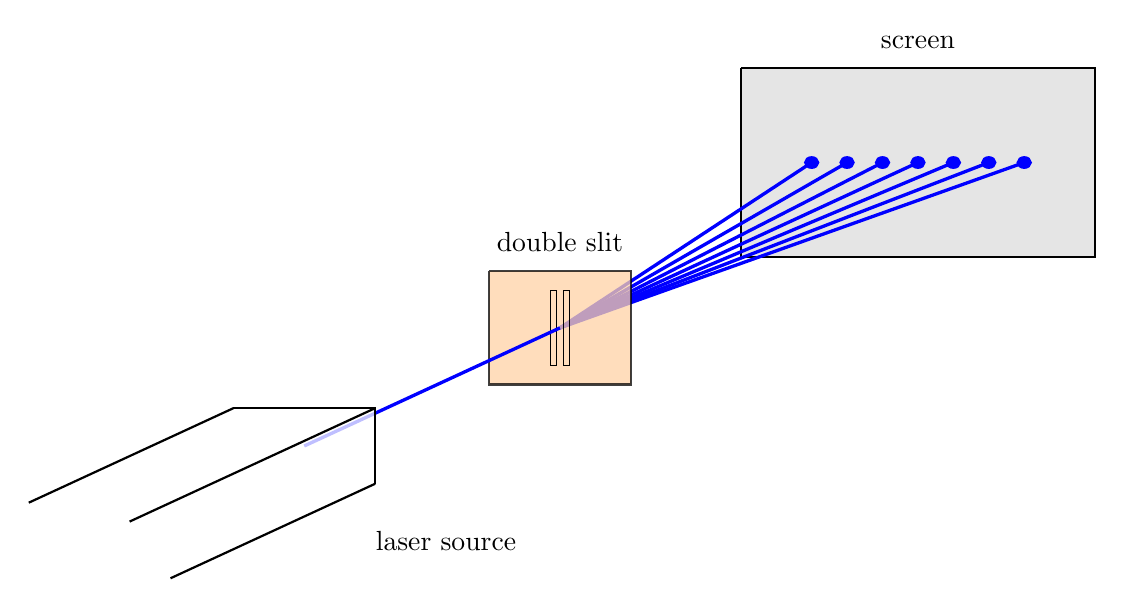
\begin{tikzpicture}[xscale=1.5, yscale=1.2]
	% screen & fringes
	\draw[thick, fill=gray!20] (30:6) ++ (-1.5,1) --++ (3,0) --++ (0,-2) --++ (-3,0) --++ (0,2);
	\foreach \x in {-0.9,-0.6,...,0.9} \draw[very thick, blue, fill] (30:6) ++ (\x, 0) circle (0.05) -- (30:2.5);
	% double slit
	\draw[thick,fill=orange!35, opacity=0.75] (30:2.5) ++ (-0.6,0.6) --++ (1.2,0) --++ (0,-1.2) --++ (-1.2,0) --++ (0,1.2);
	\draw[thin] (30:2.5) ++ (-0.08,0.4) --++ (0.05,0) --++ (0,-0.8) --++ (-0.05,0) --++ (0,0.8);
	\draw[thin] (30:2.5) ++ (0.08,0.4) --++ (-0.05,0) --++ (0,-0.8) --++ (0.05,0) --++ (0,0.8);
	\draw[very thick, blue] (30:2.5) -- (0,0);
	% laser source
	\draw[white, fill, opacity=0.75] (-0.6, 0.4) rectangle (0.6,-0.4);
	\draw[thick] (-0.6, 0.4) -- (0.6, 0.4) -- (0.6,-0.4);
	\draw[thick] (-0.6, 0.4) --++ (210:2);
	\draw[thick] (0.6,-0.4) --++ (210:2);
	\draw[thick] (0.6, 0.4) --++ (210:2.4);
	% nodes
	\draw (1.2,-1) node {laser source};
	\draw (30:6) ++ (0, 1.1) node[above] {screen};
	\draw (30:2.5) ++ (0, 0.7) node[above] {double slit};
	\end{tikzpicture}
	\caption*{Young's double-slit interference experiment}
\end{figure}


\cmt when waves from the two slits meet with path difference $\Delta L = 0, \, \lambda, \, 2\lambda, \cdots$, maxima is formed

these give positions where bright fringes are observed

\cmt when waves from the two slits meet with path difference $\Delta L = \frac{1}{2}\lambda, \, \frac{3}{2}\lambda, \, \frac{5}{2}\lambda, \cdots$, minima is formed

these give positions is where dark fringes are observed

\cmt slit-to-screen distance is usually much larger than the slit separation, i.e., $D \gg d$

in this case, bright fringes are nearly equally spaced with a separation of: \begin{empheq}[box=\tcbhighmath]{equation*}{x = \frac{\lambda D}{d}}\end{empheq}

where $d$ is separation of the two slits, $D$ is slit-to-screen distance

\begin{figure}[htp]
	\centering
	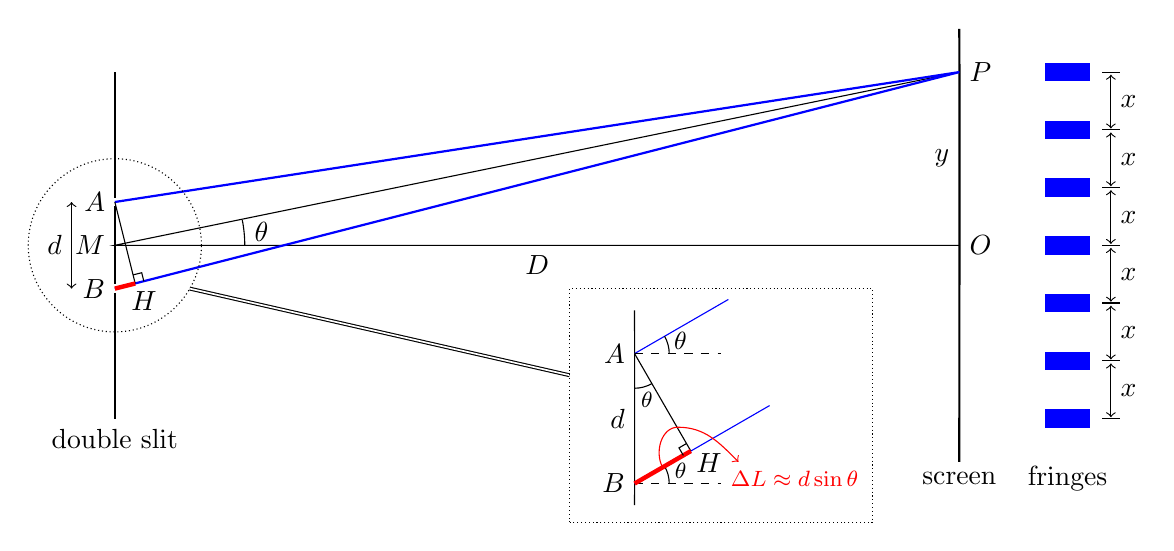
\begin{tikzpicture}[scale=0.55]
	\coordinate (A) at (0,1); \node[left] at (A) {$A$};
	\coordinate (B) at (0,-1); \node[left] at (B) {$B$};
	\coordinate (O) at (19.5,0);
	\coordinate (P) at (19.5,4);
	% double slit and screen
	\draw[thick] (0,4) -- (0,1.1) (0,0.9) -- (0,-0.9) (0,-1.1) -- (0,-4) node[below]{double slit};
	\draw (P) -- (0,0) node[left]{$M$} -- (O) node[midway,below]{$D$};
	\draw[thick] (19.5,5) -- (P) node[right] {$P$} -- (O) node[right] {$O$} node[midway,left]{$y$} -- (19.5,-5) node[below]{screen};
	% fringes
	\foreach \z in {-4, -2.667, -1.333, 0 , 1.333 ,2.667, 4}{
		\draw[blue,fill] (21.5,\z-0.2) rectangle (22.5,\z+0.2);
		\draw (22.8,\z) -- (23.2,\z);	
	}
	\foreach \z in {-4, -2.667, -1.333, 0 , 1.333 ,2.667}
	\draw[<->] (23,\z+0.03) -- (23,\z+1.273) node[midway,right]{$x$};
	\draw (22,-4.88) node[below] {fringes};
	% paths
	\draw[<->] (-1,1) -- (-1,-1) node[midway,left]{$d$};
	\draw[thick,blue] (A) -- (P) -- (B);
	\draw (0,1) -- (0.4706,-0.8824);
	\draw (0.4706,-0.8824) ++ (-0.05,0.2) -- ++(0.2,0.05) -- ++(0.05,-0.2) node[below]{$H$};
	\draw[ultra thick, red] (B) -- (0.4706,-0.8824);
	% zoom-in view
	\draw (3,0) arc(0:11.3:3); \node[right] at (3,0.32) {$\theta$};
	\draw[densely dotted] (0,0) circle(2);
	\draw[double] (-30:2) -- (10.5,-3);
	\coordinate (A') at (12,-2.5);
	\coordinate (B') at (12,-5.5);
	\draw (12,-1.5) -- (A') node[left] {$A$} -- (B') node[left]{$B$} node[midway,left]{$d$} -- (12,-6);
	\draw[blue] (A') -- ++(30:2.5);
	\draw[blue] (B') -- ++(30:3.6);
	\draw (A') -- ++(-60:2.598);
	\draw[dashed] (A') -- ++(2,0);
	\draw (A') ++ (.8,0) arc(0:30:.8);
	\draw (A') ++ (15:1.1) node{\small$\theta$};
	\draw[dashed] (B') -- ++(2,0);
	\draw (B') ++ (.8,0) arc(0:30:.8);
	\draw (B') ++ (15:1.1) node{\footnotesize$\theta$};
	\draw (A') ++ (0,-.8) arc(270:300:0.8);
	\draw (A') ++ (285:1.1) node{\footnotesize$\theta$};
	\draw[ultra thick,red] (B') -- ++(30:1.5);
	\draw (B') ++(30:1.3) -- ++(120:0.2) -- ++(30:0.2) node[below right]{$H$};
	\draw[red,->] (B') ++(30:.75) to[out=120,in=180] (13,-4.2) to[out=0,in=135] (14.4,-5);
	\draw[red] (14,-5.4) node[right] {\footnotesize{$\Delta L \approx d\sin\theta$}};
	\draw[densely dotted] (10.5,-6.4) rectangle (17.5,-1);
	\end{tikzpicture}
	
\end{figure}

\noindent \textbf{proof}: consider a point $P$ on the screen where a bright fringe is formed (see graph)

path difference between the slits must be a whole number of wavelength: $ \Delta L = \big|PB-PA\big| = n\lambda $

since $D \gg d$, paths $PA$ and $PB$ can be considered approximately parallel

so path difference is length of the segment $HB$, then we have: $\Delta L \approx d\sin\theta$

in terms of $\theta$, bright fringes are found where: $ d\sin\theta = n\lambda $

to convert $\theta$ into the coordinate $y$, we have: $\tan \theta = \frac{y}{D}$

but $\theta$ is very small, small-angle approximation ($\sin \theta \approx \tan \theta$) can be applied

so positions where the bright fringes show up are: $ y_n =  n \times \frac{\lambda D}{d} $

here the coordinate subscript $n$ labels the order of the bright fringes

this shows that the $(n+1)$-th fringe is at a fixed distance from the $n$-th fringe

therefore separation between neighbouring bright fringes is $ {x=\frac{\lambda D}{d}} $ \eoe

\cmt altering width of slit could cause a change in \emph{brightness} of fringes

width of slit determines intensity of emergent light passing through that slit

resultant amplitude will be affected as a consequence of the superposition principle

\example{A teacher demonstrates the double-slit experiment with a beam of red light produced from a helium-neon laser. The beam of wavelength of 632 nm is sent through a double-slit separated by 0.30 mm and passed onto a wall at about 2.0 m from the slits. (a) What is the fringe separation? (b) If the experiment is carried out using a green laser, what changes do you expect?}

\begin{soln} fringe separation: $ x = \frac{\lambda D}{d} = \frac{632 \times 10^{-9} \times 2.0 }{0.30 \times 10^{-3}} \RA x \approx 4.2 \times 10^{-3} \text{ m}$

if replaced by green light, wavelength becomes shorter, so smaller fringe separation \end{soln}


\example{Coherent light passes through a double slit. Initially, the light intensity from each slit is the same. State the change to the appearance of the fringes if (a) the separation between the slits is increased, (b) The width of one of the slits is reduced.}

\begin{soln} (a) from $ x = \frac{\lambda D}{d} $, shorter $\lambda$ results in smaller fringe separation

\hspace*{1.25em} but brightness of the fringes remains unchanged

(b) reducing width of slit causes amplitude of light from that slit to decrease

\hspace*{1.25em} at maxima, resultant amplitude decreases, so bright fringes become less bright

\hspace*{1.25em} at minima, amplitudes do not cancel completely, so dark fringes become a bit brighter

\hspace*{1.25em} but no change to separation between fringes \end{soln}



\subsection{multi-slit interference: diffraction gratings}

passing light through even more slits also produces nice interference patterns

\keypoint{diffraction grating} is such an apparatus, with hundreds or thousands of slits per mm\index{diffraction grating}

\begin{figure}[ht]
	\centering
	\begin{tikzpicture}[xscale=1, yscale=0.84]
	% screen & fringes
	\draw[thick, fill=gray!20] (30:7.5) ++ (-3.2,1) --++ (6.4,0) --++ (0,-2) --++ (-6.4,0) --++ (0,2);
	\foreach \x/\order in {-2.5/2,-1/1,0/0,1/1,2.5/2} \draw[very thick, blue, fill] (30:7.5) ++ (\x, 0) circle (0.05) node[black, above] {{\footnotesize $n=\order$}}-- (30:2);
	% diffraction grating
	\draw[thick,fill=orange!35, opacity=0.75] (30:2) ++ (-0.6,0.6) --++ (1.2,0) --++ (0,-1.2) --++ (-1.2,0) --++ (0,1.2);
	\foreach \x in {0.2,0.16,...,-0.2}
	\draw[ultra thin] (30:2) ++ (-\x-0.01,0.4) --++ (0.02,0) --++ (0,-0.8) --++ (-0.02,0) --++ (0,0.8);
	\draw[very thick, blue] (30:2) -- (0,0);
	% laser source
	\draw[white, fill, opacity=0.75] (-0.6, 0.4) rectangle (0.6,-0.4);
	\draw[thick] (-0.6, 0.4) -- (0.6, 0.4) -- (0.6,-0.4);
	\draw[thick] (-0.6, 0.4) --++ (210:2);
	\draw[thick] (0.6,-0.4) --++ (210:2);
	\draw[thick] (0.6, 0.4) --++ (210:2.4);
	% nodes
	\draw (1.2,-1) node {laser source};
	\draw (30:7.5) ++ (0, 1.1) node[above] {screen};
	\draw (30:2) ++ (0, 0.7) node[above, twoline] {diffraction\\grating};
	\end{tikzpicture}
	\caption*{multi-slit interference as light passes through a diffraction grating}
\end{figure}

\cmt compared to double-slit, maxima produced by diffraction grating are \emph{sharper} and \emph{brighter}

maxima are formed when waves from not two but many slits interfere constructively

\cmt location of each maxima from a diffraction grating is given by: \begin{empheq}[box=\tcbhighmath]{equation*}{d \sin \theta = n\lambda}\end{empheq}

where $d$ is the separation between adjacent slits, and light is incident \emph{normally}

\begin{figure}[htp]
	\noindent
	\centering
	\begin{minipage}{0.64\textwidth}
		\centering
		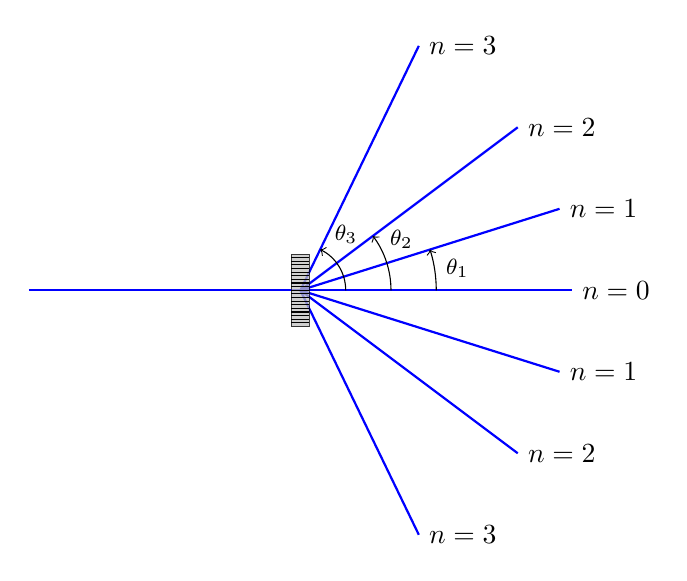
\begin{tikzpicture}[scale=1.15]
		\draw[blue,thick] (-3,0) -- (3,0) node[right] {\textcolor{black}{$n=0$}};
		\foreach \x in {1,2,3}{
			\pgfmathsetmacro{\y}{asin(\x*0.3)}
			\draw[blue,thick] (-\y:3) node[right] {\textcolor{black}{$n=\x$}} -- (0,0) -- (\y:3) node[right] {\textcolor{black}{$n=\x$}};
			\draw[->] ({2-\x*0.5}, 0) arc (0:\y:{2-\x*0.5});
		}
		\draw[fill=gray!50, opacity=0.75] (-0.1,-0.4) rectangle (0.1,0.4);
		\foreach \y in {0.36,0.32,...,-0.36} \draw (-0.1,\y) -- (0.1,\y);
		\node at (8:1.75) {{\footnotesize $\theta_1$}};
		\node at (27:1.25) {{\footnotesize $\theta_2$}};
		\node at (51:0.8) {{\footnotesize $\theta_3$}};
		\end{tikzpicture}
	\end{minipage}\hfill
	\begin{minipage}{0.35\textwidth}
		\centering
		\begin{tikzpicture}[scale=1.3]
		\foreach \y in {0,1,2,3,4}
		\draw[ultra thick] (0,\y+0.1) -- (0,\y+0.9);
		\foreach \y in {1,2,3,4}{
			\draw[blue] (0,\y) -- ++(30:2);
			\draw (-0.3,\y) -- (-0.7,\y);
		}
		\foreach \y in {2,3,4}{
			\draw[<->] (-0.5,\y-0.97) -- (-0.5,\y-0.03) node[midway,left]{$d$};
			\draw (0,\y) -- ++(-60:.866);
			\draw[very thick, red] (0,\y-1) -- ++(30:.5);
			\draw[red, decoration={markings,mark=at position 1 with {\arrow[scale=2]{>}}},
			postaction={decorate},dashed] (0,\y-1) -- ++(30:.25) to[out=-45,in=135] (2,1);
			\draw (0,\y-.3) arc(270:300:.3);
			\draw (0,\y) ++ (285:.5) node {\footnotesize$\theta$};
		}
		\node[below] at (2,1) {$\Delta L = d\sin\theta$};
		\end{tikzpicture}
	\end{minipage}
\end{figure}

\noindent\textbf{proof} for constructive interference, path difference between adjacent slits must satisfy: $\Delta L = n\lambda $

since slits are so close together, light rays passing through the slits are nearly parallel

using the same trick as before, we obtain: $d \sin \theta = n\lambda$

this is known as the \emph{diffraction grating equation}.



\cmt greatest angle through which a beam of light can be diffracted is 90$^\circ$

this puts a constraint on the highest order possible:
\begin{equation*}
n_\tmax = \frac{d\sin\theta_\tmax}{\lambda} < \frac{d \sin 90^\circ}{\lambda} \RA \boxed{n_\tmax < \frac{d}{\lambda}}
\end{equation*}

the value of $\frac{d}{\lambda}$ should be rounded \emph{down} to the nearest whole number to give $n_\tmax$

\cmt if white light is passed through diffraction gratings, \emph{dispersion} is observed

\begin{figure}[!ht]
	\centering
	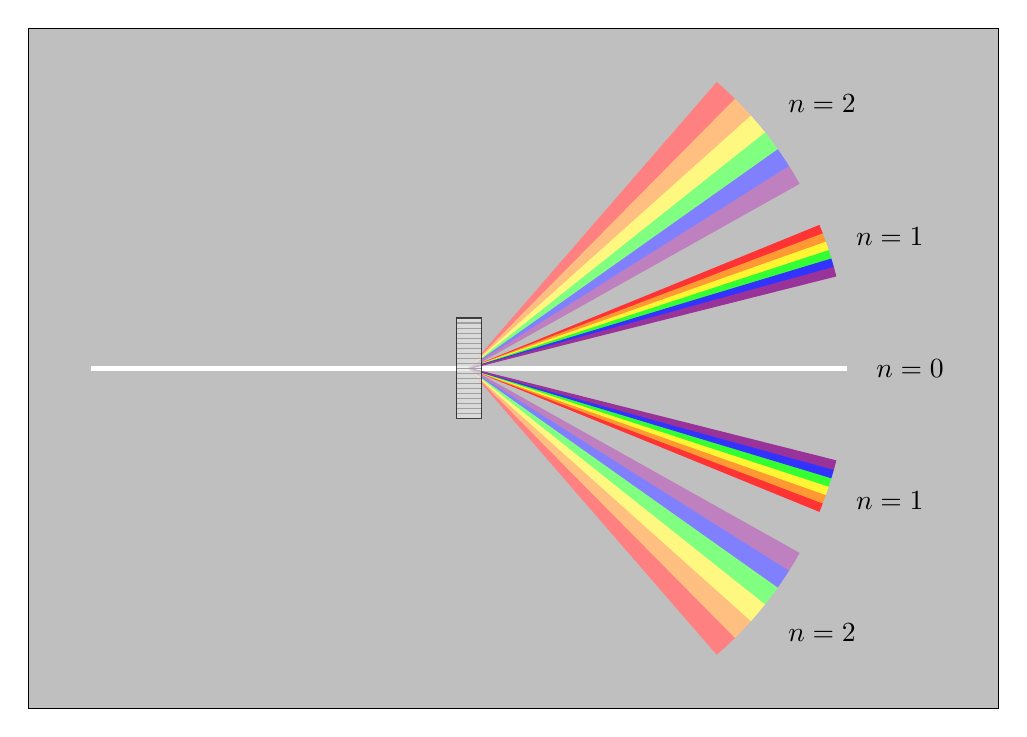
\begin{tikzpicture}[scale=1.6]
	% background
	\draw[fill=gray!50] (-3.5,-2.7) rectangle (4.2,2.7);
	% zeroth order
	\draw[white,ultra thick] (-3,0) -- (3,0);
	% first and second order
	\foreach \WL/\yanse in {6.4/red, 6.0/orange, 5.6/yellow, 5.2/green, 4.8/blue, 4.4/violet}{
		\pgfmathsetmacro{\ystart}{asin(\WL/18)}
		\pgfmathsetmacro{\yend}{asin((\WL+0.4)/18)}
		\draw[\yanse!80, fill] (0,0) -- (\ystart:3) arc(\ystart:\yend:3) -- cycle;
		\draw[\yanse!80, fill] (0,0) -- (-\ystart:3) arc(-\ystart:-\yend:3) -- cycle;
		\pgfmathsetmacro{\zstart}{asin(\WL/9)}
		\pgfmathsetmacro{\zend}{asin((\WL+0.4)/9)}
		\draw[\yanse!50, fill] (0,0) -- (\zstart:3) arc(\zstart:\zend:3) -- cycle;
		\draw[\yanse!50, fill] (0,0) -- (-\zstart:3) arc(-\zstart:-\zend:3) -- cycle;
	}
	% order labels
	\foreach \t/\nlabel in {0/0, 5.4/1, 10.8/2, -5.4/1, -10.8/2}{
		\pgfmathsetmacro{\y}{asin(\t/18)}
		\node at (\y:3.5) {$n=\nlabel$};
	}
	% diffraction grating
	\foreach \y in {0.36,0.32,...,-0.36} \draw (-0.1,\y) -- (0.1,\y);
	\draw[fill=gray!20, opacity=0.7] (-0.1,-0.4) rectangle (0.1,0.4);
	\end{tikzpicture}
	\caption*{dispersion of white light through a diffraction grating}
\end{figure}



\newpage

\begin{compactitem}
	\item[--] at zeroth order, diffraction grating equation $d\sin\theta_0 = 0\cdot\lambda$ is satisfied at $\theta_0 = 0$ for any $\lambda$
	
	so we observe a collection of all colours, i.e., a white central maxima
	
	\item[--] at first order, $d\sin\theta_1 = 1\cdot\lambda$, maxima for long wavelengths appear at greater angles
	
	spectrum spreads into a rainbow band, with red light at outer end and violet closer in
	
	\item[--] at higher orders, dispersion would be more spread out 
	
	the spectra of different orders may even overlap to give complicated combinations
	
	we do not intend to discuss this further
\end{compactitem}

\cmt diffraction grating is an import device in analysis of light

it is widely used in measurement of wavelength of light

\example{Light of 632 nm wavelength produces first-order maxima at 16$^\circ$ when passing through a diffraction grating at right angles. How many lines per millimetre are there in the diffraction grating?}

\begin{soln} slit separation: $d = \frac{n\lambda}{\sin\theta} = \frac{1\times632\times10^{-9}}{\sin 16^\circ} \RA d \approx 2.29 \times 10^{-6} \text{ m}$

number of lines in 1 mm: $N = \frac{1 \text{ mm}}{2.29 \times 10^{-6} \text{ m}} = \frac{1 \times 10^{-3}}{2.29 \times 10^{-6}} \RA N \approx 436$ \end{soln}

\example{Green light of 510 nm wavelength is incident normally on a diffraction grating with slit separation of 2.0 $\mu$m. (a) What is the highest order seen? (b) how many maxima are produced? (c) If blue light is used for the same diffraction grating experiment, suggest the effect on the diffraction pattern.}

\begin{soln} to find highest order, we have: $n_\tmax < \frac{d\sin 90^\circ}{\lambda} = \frac{2.0\times10^{-6}}{510\times10^{-9}} \approx 3.9 \RA n_\tmax = 3$

1st, 2nd, 3rd-order on either side and 0th-order at centre, so $ 2\times 3 + 1 = 7$ maxima are formed

blue light has shorter wavelength, so more maxima will be produced with blue light, and separation between each maxima would be closer \end{soln}

\example{Light of wavelength 630 nm produces a second-order maxima at angle of $60^\circ$ when it is directed at a diffraction grating. If visible light of another wavelength can also give a maximum at the same angle, what is this wavelength?}

\begin{soln} using diffraction grating equation: $d \sin\theta = n\lambda$, we find $n\lambda$ is constant for fixed $\theta$

from information given in the question, this constant is $ 2\times630 = 1260 \text{ nm}$

if $n=1$, $\lambda = 1260 \text{ nm}$, which would be infra-red

if $n=3$, $\lambda = 420 \text{ nm}$, which would be visible (violet)

if $n\geq 4$, $\lambda \leq 315 \text{ nm}$, which would be ultraviolet

so the desired wavelength is 420 nm \end{soln}







\subsection{stationary waves}

\subsection{formation of stationary waves}

stationary waves are often formed when a travelling wave is \emph{reflected} at a some point

forward-moving wave and backward-moving reflected wave combine to form stationary wave

\begin{ilight}
	when two waves of same frequency and same speed travel in opposite directions and meet together, they superpose to form stable regions of constructive and destructive interference, this forms a \keypoint{stationary wave}, also known as a \keypoint{standing wave}\index{stationary wave}
\end{ilight}

\begin{figure}[htp]
	\centering
	\noindent\begin{minipage}{0.25\linewidth}
		\centering
		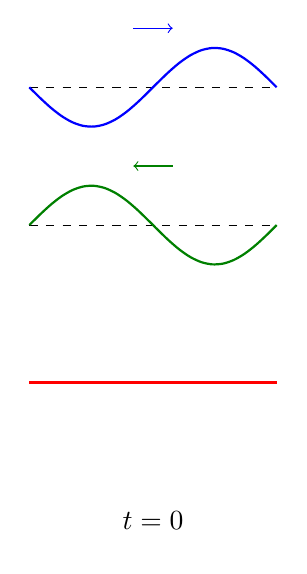
\begin{tikzpicture}[scale=0.5]
		\foreach \y in {0, -3.5, -7.5}
		\draw[thin, dashed] (-pi, \y) -- (pi, \y);
		\draw [thick,blue,domain=-pi:pi,samples=24,smooth,variable=\x] plot (\x,{sin(\x r)});
		\draw[->,blue] (-0.5,1.5) -- (0.5,1.5);
		\draw [thick,Green,domain=-pi:pi,samples=24,smooth,variable=\x] plot (\x,{sin(-\x r)-3.5});
		\draw[<-,Green] (-0.5,1.5-3.5) -- (0.5,1.5-3.5);
		\draw [very thick,red,domain=-pi:pi,samples=5,smooth,variable=\x] plot (\x,{-7.5});
		\node at (0,-11) {$t=0$};
		\node[white] at (2,-11) {$\frac{1}{1}$};
		\end{tikzpicture}
	\end{minipage}\hfil
	\begin{minipage}{0.25\linewidth}
		\centering
		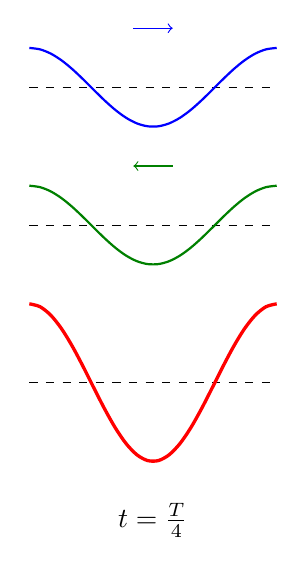
\begin{tikzpicture}[scale=0.5]
		\foreach \y in {0, -3.5, -7.5}
		\draw[thin, dashed] (-pi, \y) -- (pi, \y);
		\draw [thick,blue,domain=-pi:pi,samples=24,smooth,variable=\x] plot (\x,{-cos(\x r)});
		\draw[->,blue] (-0.5,1.5) -- (0.5,1.5);
		\draw [thick,Green,domain=-pi:pi,samples=24,smooth,variable=\x] plot (\x,{-cos(\x r)-3.5});
		\draw[<-,Green] (-0.5,1.5-3.5) -- (0.5,1.5-3.5);
		\draw [very thick,red,domain=-pi:pi,samples=24,smooth,variable=\x] plot (\x,{-2*cos(\x r)-7.5});
		\node at (0,-11) {$t=\frac{T}{4}$};
		\end{tikzpicture}
	\end{minipage}\hfil
	\begin{minipage}{0.25\linewidth}
		\centering
		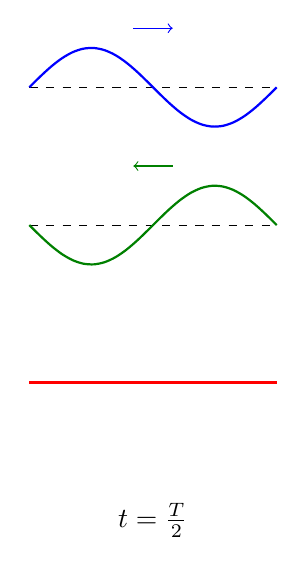
\begin{tikzpicture}[scale=0.5]
		\foreach \y in {0, -3.5, -7.5}
		\draw[thin, dashed] (-pi, \y) -- (pi, \y);
		\draw [thick,blue,domain=-pi:pi,samples=24,smooth,variable=\x] plot (\x,{-sin(\x r)});
		\draw[->,blue] (-0.5,1.5) -- (0.5,1.5);
		\draw [thick,Green,domain=-pi:pi,samples=24,smooth,variable=\x] plot (\x,{-sin(-\x r)-3.5});
		\draw[<-,Green] (-0.5,1.5-3.5) -- (0.5,1.5-3.5);
		\draw [very thick,red,domain=-pi:pi,samples=5,smooth,variable=\x] plot (\x,{-7.5});
		\node at (0,-11) {$t=\frac{T}{2}$};
		\end{tikzpicture}
	\end{minipage}\hfil
	\begin{minipage}{0.25\linewidth}
		\centering
		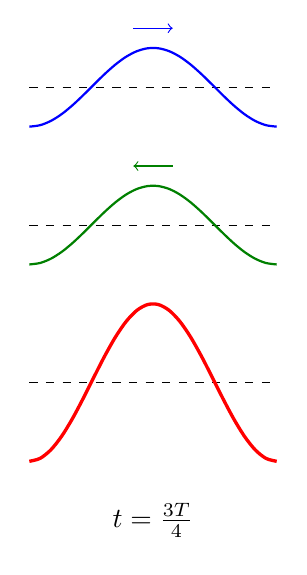
\begin{tikzpicture}[scale=0.5]
		\foreach \y in {0, -3.5, -7.5}
		\draw[thin, dashed] (-pi, \y) -- (pi, \y);
		\draw [thick,blue,domain=-pi:pi,samples=24,smooth,variable=\x] plot (\x,{cos(\x r)});
		\draw[->,blue] (-0.5,1.5) -- (0.5,1.5);
		\draw [thick,Green,domain=-pi:pi,samples=24,smooth,variable=\x] plot (\x,{cos(\x r)-3.5});
		\draw[<-,Green] (-0.5,1.5-3.5) -- (0.5,1.5-3.5);
		\draw [very thick,red,domain=-pi:pi,samples=24,smooth,variable=\x] plot (\x,{2*cos(\x r)-7.5});
		\node at (0,-11) {$t=\frac{3T}{4}$};
		\end{tikzpicture}
	\end{minipage}
	
	\vspace*{0.75em} formation of a stationary wave (red) due to the superposition of one wave 
	
	travelling to the right (blue) and another wave travelling to the left (green)
\end{figure}

from this one can visualise how the pattern of a stationary wave varies with time

\begin{figure}[htp]
	\centering
	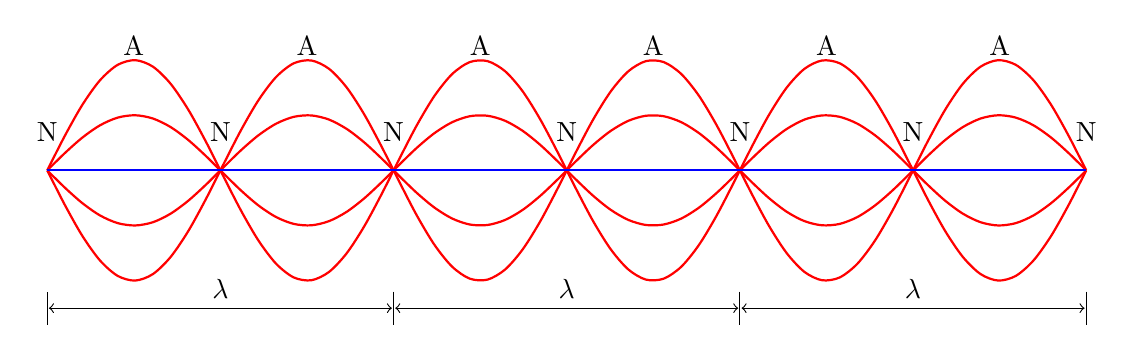
\begin{tikzpicture}[scale=0.7]
	\foreach \amp in {-2,-1,1,2}
	\draw [thick,red,domain=-3*pi:3*pi,samples=60,smooth,variable=\x] plot (\x,{\amp*sin(\x r)});
	\draw [thick,blue] (-3*pi,0) -- (3*pi,0);
	\foreach \idx in {-1,0,1}{
		\draw[<->] (\idx*2*pi-pi+0.03,-2.5) -- ++(2*pi-0.06,0) node[midway,above]{$\lambda$};
		\draw (\idx*2*pi-pi,-2.8) -- ++(0,0.6) ++(2*pi,0) -- ++(0,-0.6);
	}
	\foreach \n in {-3,-2,...,3} \node at (\n*pi,0.7) {N};
	\foreach \a in {-2.5,-1.5,...,2.5} \node at (\a*pi,2.25) {A};
	\end{tikzpicture}
	\caption*{variation of a stationary wave pattern with time}
\end{figure}

\cmt there are points in the wave where destructive interference always occurs

these points are called \keypoint{nodes}, which have zero amplitudes \index{node}

\cmt points oscillating with the greatest amplitudes are called \keypoint{anti-nodes} \index{anti-node}

\cmt points other than nodes and anti-nodes oscillate with different amplitudes

\cmt distance between two adjacent nodes is half of one wavelength

wavelength can be estimated as: \begin{empheq}[box=\tcbhighmath]{equation*}{\lambda = 2 \times \text{node-to-node distance}}\end{empheq}



\subsection{stationary wave pattern \& boundary conditions}

patterns of stationary waves depend heavily on the boundary conditions

\cmt the end can be \emph{fixed}, also called a \emph{closed} end, to form a \emph{node}

\cmt the end can also be \emph{free} to oscillate, known as an \emph{open} end, to form \emph{an anti-node}



\subsection*{stationary wave between two fixed ends}

with both ends fixed, the two ends are both nodes

three patterns with the longest wavelengths and lowest frequencies are shown

\begin{figure}[htp]
	\centering
	\noindent\begin{minipage}{0.3\linewidth}
		\centering
		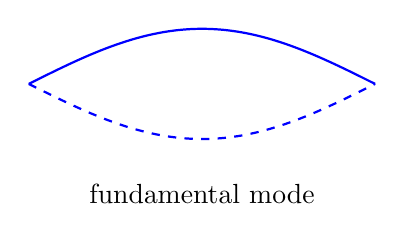
\begin{tikzpicture}[scale=0.7]
		\draw [thick,blue,domain=-pi:pi,samples=24,smooth,variable=\x] plot (\x,{cos(\x/2 r)});
		\draw [thick,dashed,blue,domain=-pi:pi,samples=24,smooth,variable=\x] plot (\x,{-cos(\x/2 r)});
		\node at (0,-2) {fundamental mode};
		\end{tikzpicture}
	\end{minipage}\hfil
	\begin{minipage}{0.3\linewidth}
		\centering
		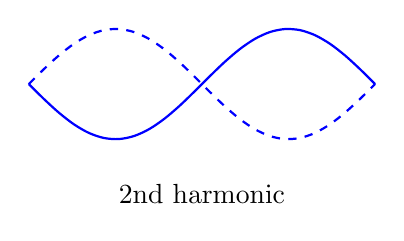
\begin{tikzpicture}[scale=0.7]
		\draw [thick,blue,domain=-pi:pi,samples=24,smooth,variable=\x] plot (\x,{sin(\x r)});
		\draw [thick,dashed,blue,domain=-pi:pi,samples=24,smooth,variable=\x] plot (\x,{-sin(\x r)});
		\node at (0,-2) {2nd harmonic};
		\end{tikzpicture}
	\end{minipage}\hfil
	\begin{minipage}{0.3\linewidth}
		\centering
		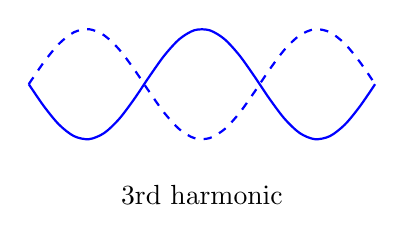
\begin{tikzpicture}[scale=0.7]
		\draw [thick,blue,domain=-pi:pi,samples=24,smooth,variable=\x] plot (\x,{cos(3*\x/2 r)});
		\draw [thick,dashed,blue,domain=-pi:pi,samples=24,smooth,variable=\x] plot (\x,{-cos(3*\x/2 r)});
		\node at (0,-2) {3rd harmonic};
		\end{tikzpicture}
	\end{minipage}\hfil
\end{figure}

\cmt longest-wavelength mode is called the \emph{fundamental mode}, it also has lowest frequency

modes with higher frequencies are usually referred to as \emph{excited modes}, or \emph{harmonics}\footnote{These modes are closely related to the notes played on musical instruments.}

in many texts different modes are labelled as 1st, 2nd, 3rd \emph{harmonics}, etc.

\cmt if two ends are separated by a distance of $L$, then wavelengths for different modes are:
\begin{equation*}
\lambda_1 = 2L \qquad \lambda_2 = L \qquad \lambda_3 = \frac{2L}{3} \qquad \cdots \qquad \lambda_n = \frac{2L}{n}
\end{equation*}

making comparison with the fundamental wavelength $\lambda_1$ $\lambda_1$, we have
\begin{equation*}
\lambda_2 = \frac{\lambda_1}{2} \qquad \lambda_3 = \frac{\lambda_1}{3} \qquad \cdots \qquad \lambda_n = \frac{\lambda_1}{n}
\end{equation*}

\cmt since wave speed remains constant as wave travels through the same medium

frequency of each mode is inversely proportional to its wavelength, hence,  
\begin{equation*}
f_2 = 2f_1 \qquad f_3 = 3f_1 \qquad \cdots \qquad f_n=n f_1
\end{equation*}

\example{\emph{Melde's experiment} demonstrates a stationary wave formed on a vibrating string using an oscillator set at a particular frequency. Given that the length of the string is 80 cm. (a) What is the wavelength of this wave? (b) If one wants to construct a stationary of longer wavelength, suggest what changes can be made?}

\begin{figure}[ht]
	\centering
	\begin{tikzpicture}[scale=1.1]
	\draw [thick,domain=0:10,samples=90,smooth] plot (\x,{.6*sin(\x*90)});
	\draw [thick,domain=0:10,samples=90,smooth] plot (\x,{-.6*sin(\x*90)});
	\draw[fill] (0,0) circle (0.1);
	\draw[fill] (10,0) circle (0.1);
	\draw[thick] (10,-1) -- (10,1);
	\foreach \y in {0.9,0.6,...,-0.7} \draw (10,\y) --++ (0.2,-0.2);
	\draw (-0.03, 0) rectangle (0.03, -1);
	\draw[thick] (-.8, -1) rectangle (.8,-2);
	\node at (0,-1.5) {oscillator};
	\node[twoline, right] at (10.2, 0) {fixed\\point};
	\end{tikzpicture}
	\caption*{Melde's experiment: demonstration of stationary waves on a tense string}
\end{figure}

\begin{soln} five loops so five half-wavelengths $\RA L = \frac{5}{2}\lambda \RA \lambda = \frac{2}{5}L = \frac{2}{5} \times 80 \RA \lambda = 32\text{ cm}$

to have larger wavelength, one could do either of the following:
use a string with greater length (while keeping frequency of oscillator unchanged)
reduce the frequency of oscillation (constant wave speed, so $\lambda$ increases)

\titem increase tension in string (wave speed increases \end{soln}\footnote{The speed $v$ of a progressive wave travelling along a string of length $L$ and mass $m$ can be given by the equation: $v = \sqrt{\frac{TL}{m}}$, where $T$ is the tension in the string.} for same frequency, so $\lambda$ increases)




\subsection*{stationary wave between one fixed end and one open end}

in this case, we have a node at one end and an anti-node at the other end

again we give the three patterns with the longest wavelengths and lowest frequencies

\begin{figure}[htp]
	\centering
	\noindent\begin{minipage}{0.3\linewidth}
		\centering
		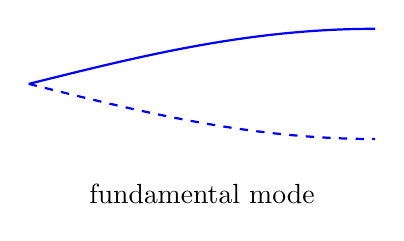
\begin{tikzpicture}[scale=0.7]
		\draw [thick,blue,domain=0:2*pi,samples=24,smooth,variable=\x] plot (\x,{sin(\x/4 r)});
		\draw [thick,dashed,blue,domain=0:2*pi,samples=24,smooth,variable=\x] plot (\x,{-sin(\x/4 r)});
		\node at (pi,-2) {fundamental mode};
		\end{tikzpicture}
	\end{minipage}\hfil
	\begin{minipage}{0.3\linewidth}
		\centering
		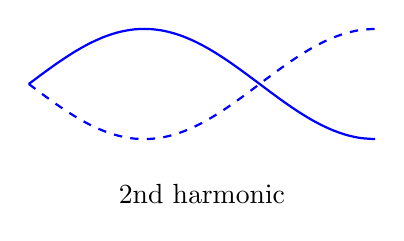
\begin{tikzpicture}[scale=0.7]
		\draw [thick,blue,domain=0:2*pi,samples=24,smooth,variable=\x] plot (\x,{sin(3*\x/4 r)});
		\draw [thick,dashed,blue,domain=0:2*pi,samples=24,smooth,variable=\x] plot (\x,{-sin(3*\x/4 r)});
		\node at (pi,-2) {2nd harmonic};
		\end{tikzpicture}
	\end{minipage}\hfil
	\begin{minipage}{0.3\linewidth}
		\centering
		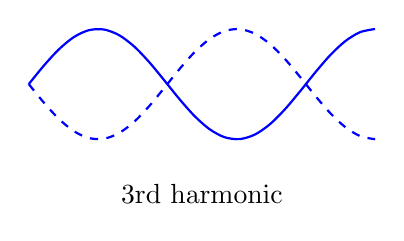
\begin{tikzpicture}[scale=0.7]
		\draw [thick,blue,domain=0:2*pi,samples=24,smooth,variable=\x] plot (\x,{sin(5*\x/4 r)});
		\draw [thick,dashed,blue,domain=0:2*pi,samples=24,smooth,variable=\x] plot (\x,{-sin(5*\x/4 r)});
		\node at (pi,-2) {3rd harmonic};
		\end{tikzpicture}
	\end{minipage}\hfil
%	\caption{The three lowest frequency modes of wave patterns formed between one fixed end and one open end}
\end{figure}

\cmt longest-wavelength/lowest-frequency mode is also called the \emph{fundamental mode}

excited modes are called \emph{harmonics} as before

\cmt wavelengths for allowed patterns under the boundary conditions are
\begin{equation*}
\lambda_1 = 4L \qquad \lambda_2 = \frac{4L}{3} \qquad \lambda_3 = \frac{4L}{5} \qquad \cdots \qquad \lambda_n = \frac{4L}{2n-1}
\end{equation*}

comparing with the fundamental wavelength $\lambda_1$, we find
\begin{equation*}
\lambda_2 = \frac{\lambda_1}{3} \qquad \lambda_3 = \frac{\lambda_1}{5} \qquad \cdots \qquad \lambda_n = \frac{\lambda_1}{2n-1}
\end{equation*}

again the wave speed should be the same for all modes, so the allowed frequencies are
\begin{equation*}
f_2 = 3f_1 \qquad f_3 = 5f_1 \qquad \cdots \qquad f_n=(2n-1) f_1
\end{equation*}

\begin{marginfigure}
	\vspace*{-5pt}
	\centering
	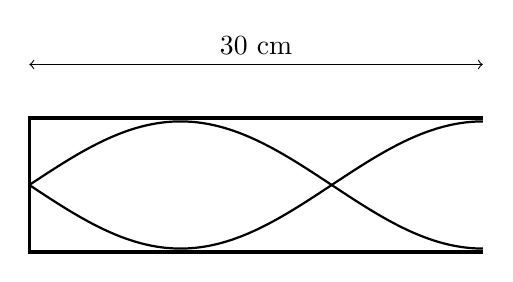
\begin{tikzpicture}[xscale=0.64, yscale=0.85]
	\draw[<->] (9,1.8) -- (0,1.8) node[midway,above]{30 cm}; 
	\draw[very thick] (9,1) -- (0,1) -- (0,-1) -- (9,-1);
	\draw [thick,domain=0:9,samples=90,smooth] plot (\x,{0.95*sin(\x*30)});
	\draw [thick,domain=0:9,samples=90,smooth] plot (\x,{-0.95*sin(\x*30)});
	\end{tikzpicture}
	\vspace*{-16pt}
\end{marginfigure}


\example{The graph shows a standing sound wave produced in an air column in a closed pipe of length 30 cm. The frequency of this sound wave is 825 Hz. (a) What is the wavelength of the sound wave? (b) Calculate the speed of sound. (c) What is the frequency of the fundamental mode for sound wave in this air column? (d) Describe the motion of an air molecule near the open end.}
	
\begin{soln} (a) wavelength of this excited mode: $\lambda = \frac{4}{3}L = \frac{4}{3}\times 30 \times 10^{-2} \RA \lambda = 0.40 \text{ m}$

(b) wave speed: $v = \lambda f = 0.40 \times 825 \RA v = 330 \mps$

(c) wavelength of fundamental mode: $\lambda = 4L = 4\times 30\times10^{-2} \RA \lambda = 1.2 \text{ m}$

\hspace*{1.25em} fundamental frequency: $f = \frac{v}{\lambda} = \frac{330}{1.2} \RA f = 275 \text{ Hz}$

(d) note that an anti-node is formed near open end, also sound wave is longitudinal

\hspace*{1.25em} so air molecule near open end vibrate \emph{horizontally} with greatest amplitude \end{soln}



\begin{marginfigure}
	\vspace*{-8pt}
	\centering
	\begin{tikzpicture}[scale=1.5]
	\draw[cyan!40, fill] (-0.5,0) rectangle (0.5, 2.5);
	\draw[cyan!40, fill] (-0.8,0.3) rectangle (-0.5, 0.6);
	\draw[thick] (-0.8, 0.3) -- (-0.5, 0.3) -- (-0.5, 0) -- (0.5, 0) -- (0.5, 4); 
	\draw[thick] (-0.8, 0.6) -- (-0.5, 0.6) -- (-0.5, 4); 
	\draw[ultra thick] (-0.4, 4.5) -- (0.3, 4.5) arc(90:-90:0.1) -- (-0.4, 4.3);
	\draw[ultra thick] (0.4, 4.4) --++ (0.4,0);
	\draw (0.6, 4.5) --++ (0.4, 0.3) node[right, twoline]{tuning\\fork};
	\draw (0.3, 2) --++ (0.6, 0.4) node[right]{water};
	\draw[thick,->] (-0.9, 0.45) --++ (-0.4,0);
	\draw[very thick] (-1,0) -- (1,0);
	\end{tikzpicture}
	\vspace*{10pt}
\end{marginfigure}


\example{A tuning fork is held above a tall cylinder which is initially filled with water. The water level, measured from the bottom of the cylinder, is lowered at a constant rate. A loud sound is first heard when the water level is at 60.0 cm, and the next loud sound is heard when the water level is at 26.8 cm. It is known that the speed of sound in air is $340 \mps$. What is the frequency of the sound wave produced by the tuning fork?}

\begin{soln} loud sound is heard when stationary wave is set up

node is formed at surface of water

node-to-node distance is $60.0 - 26.8 = 33.2 \text{ cm}$

wavelength of this wave: $\lambda = 2 \times 33.2 \text{ cm} = 0.664 \text{ m}$

frequency: $f = \frac{v}{\lambda} = \frac{340}{0.664} \RA f \approx 512 \text{ Hz}$ 
\end{soln}

\subsection*{stationary wave between two open ends}

the result is left as an exercise for the reader to prove

you shall verify that the allowed wavelengths are: $\lambda = 2L, \, L, \,\frac{2}{3}L, \cdots, \frac{2L}{n}, \cdots$

frequencies of the fundamental and excited modes go as $f = f_1, \, 2f_1, \, 3f_1, \cdots, nf_1 \cdots$


\subsection{measurement of speed of sound with stationary waves}

speed of sound waves can be measured using stationary waves as follows

\begin{figure}[ht]
	\centering
	\begin{circuitikz}
		% loudspeaker
		\draw (-0.6,0.55) to[loudspeaker, name=L] (-0.6,-0.55);
%		\node [waves, scale=0.7, right] at(L.north) {};
		\node[above] at (-0.6,0.65) {loudspeaker};
		% microphone
		\draw[thick] (5.22,0) rectangle (5.38,-0.8);
		\draw[thick, fill=white] (5.3,0) circle (0.2);
		\draw[thick] (5.3, -0.8) [out=-90, in=60] to (3.5,-2); 
		\node[above] at (5.3, 0.3) {microphone};
		\draw[thick, ->] (5.6,0) --++ (0.4,0);
		\draw[thick, ->] (5.0,0) --++ (-0.4,0);
		% oscilloscope
		\draw[thick, rounded corners] (1.9,-2) rectangle (5,-4);
		\draw[rounded corners] (2, -2.1) rectangle (4, -3.9);
		\foreach \y in {-2.4, -3, -3.6} {
			\draw[thick] (4.5, \y) circle (0.2);
		}
		\foreach \x in {2.2, 2.4, ..., 3.8} \draw[very thin, gray!40] (\x, -2.1) -- (\x, -3.9);
		\foreach \y in {-2.3, -2.5, ..., -3.7} \draw[very thin, gray!40] (2, \y) -- (4, \y);
		\draw [thick,Green, domain=2:4,samples=80,smooth] plot (\x,{0.65*sin((\x-2.7)*540) - 3});
		\node[below] at (3.5, -4.1) {oscilloscope};
		% metal plate
		\draw[thick, fill=gray!20] (9,0) ++ (-0.4,1) --++ (0.8,-0.5) --++ (0,-2) --++ (-0.8,0.5) --++ (0,2);
		\node[above] at (9, 1) {metal plate};
		% wave pattern
		\draw [gray, dashed, domain=0:9,samples=80,smooth] plot (\x,{0.3*sin(\x*80)});
		\draw [gray, dashed, domain=0:9,samples=80,smooth] plot (\x,{-0.3*sin(\x*80)});
	\end{circuitikz}
	\caption*{arrangement of apparatuses for setting up a stationary sound wave}
\end{figure}

\cmt to set up a stationary sound wave, we need two travelling waves in opposite directions

sound wave can be produced by a \emph{loudspeaker} (coupled to a \emph{signal generator})

this forward-travelling wave is reflected at a \emph{metal plate}

reflected wave superposes with wave from loudspeaker to give a stationary wave

wave intensity can be detected by a \emph{microphone} and observed on an \emph{oscilloscope}

\cmt to verify whether stationary wave is formed, we check whether nodes are formed

positions of the metal plate and the microphone are adjusted carefully

if there exists a location where no signal is detected, this means microphone is at a node

now a stationary wave has been formed between loudspeaker and reflector

\cmt to find wavelength of sound wave, we slowly move microphone to the next node

wavelength of sound wave: $\lambda = 2\times \text{distance between neighbouring nodes}$

\cmt to find frequency of sound wave, we move microphone to anywhere that is not a node

from time base of the oscilloscope, we can work out period $T$ of the wave

frequency is then given by the formula: $f=\frac{1}{T}$

\cmt finally,  speed of the sound wave\footnote{We should bear in mind that stationary waves do not propagate through space, so rigorously speaking, it is incorrect to say the speed of a stationary way. The wave speed calculated in this way refers to the speed of either of the two travelling waves that give rise to the stationary wave through superposition.} can be calculated: $v=\lambda f$




\subsection{stationary waves \& progressive waves}

there are quite a few differences between a stationary wave and a progressive wave

\cmt progressive wave can transfer energy from one place to another

but for stationary waves, vibrational energy is not transferred due to existence of nodes

\cmt different points in general have different amplitudes over a stationary wave

\hspace*{1.25em} nodes have zero amplitude, anti-nodes have greatest amplitudes

\hspace*{1.25em} other points have various amplitudes depending on their positions

but for a progressive wave, all points have the same amplitude

\hspace*{1.25em} displacements of each point at a particular moment can be all different

\hspace*{1.25em} but the largest displacements they can reach are the same (if no loss of energy)

\cmt phase difference between any two points in a progressive wave can take any value

\hspace*{1.25em} different points reach their peaks at different times for a progressive wave

\hspace*{1.25em} so $\Delta \phi$ can be anything from 0 to $2\pi$ (or anything from 0 to $360^\circ$)

phase difference between any two points in a stationary wave is either 0 or $\pi$ (or $180^\circ$)

\hspace*{1.25em} for points between adjacent nodes, they all reach their highest at same time

\hspace*{1.25em} despite differences in amplitudes, these points are all in phase, so $\Delta \phi=0$

\hspace*{1.25em} for points separated by one node, they are anti-phase

\hspace*{1.25em} this is because when one is at its peak, the other is at its trough, so $\Delta \phi = \pi$ (or $180^\circ$)


	
\subsection{end-of-chapter questions}


\subsection*{principle of superposition}

\question{
	Noise reduction headphones can cancel out external sound waves by producing their own sound waves. What is the phase difference between the external sound wave and the wave produced in the headphone?
}

\question{
	A wave of frequency of 10 Hz travels at a speed of $4.0 \mps$. What is the phase difference between two points 0.50 m apart?
}

\question{
	Two loudspeakers $A$ and $B$ are connected to the same signal generator. They give out sound signals of wavelength 0.50 m. A person stands in a position which is at a distance of 20.0 m from $A$ and 21.0 m from $B$. Initially, only loudspeaker $A$ is emitting sound. What happens to the intensity of the sound heard by the person when loudspeaker $B$ is also switched on?
}

\question{
	A students thinks that the superposition of waves is about the superposition of the wave amplitudes. Give a counter-example why he is wrong.
}

\question{
	Two separate loudspeakers generate sound waves of slightly different frequencies. (a) Explain why a stable interference is not observed. (b) If an observer stands at a fixed location, state and explain the variation of the intensity of the sound that he hears.
}

\question{
	Two waves $A$ and $B$ are of the same type. Given that they have a phase difference of $120^\circ$, and the intensity of wave $A$ is twice that of wave $B$. On the same graph, sketch the displacement against time to illustrate the two waves.
}


\question{
	Two waves $A$ and $B$ of the same amplitude have a phase difference of $90^\circ$. (a) On the same graph, sketch the displacement against time to illustrate the two waves. (b) Sketch the variation of the resultant displacement if $A$ and $B$ superpose together.
}



\subsection*{double-slit experiment}

\question{
	A laser emits a yellow light of 580 nm. It is sent through a set of double slits with a separation of 0.40 mm. An interference pattern is seen on a screen at a distance of 2.5 m from the slits. What is the distance between a bright fringe and its closest dark fringe?
}


\question{
	A double-slit interference pattern is produced on a screen using a red laser of 630 nm wavelength. The screen is 4.0 m from the double slit, and the fringes are seen to have a spacing of 15 mm. What is the separation of the slits?
}

\newpage


\question{
	Light is incident normally on two narrow slits which are of 2.00 mm apart. A screen is at a distance of 2.5 m from the slits. The distance between the central maximum and the 4$^\text{th}$ bright spot is found to be 3.2 mm. What is the wavelength of the light?
}

\question{
	In a double-slit experiment, suggest by what factor does the separation between bright fringes change if (a) the distance between the slits and the screen is doubled, (b) the slit separation is doubled, (c) the frequency of incident light is doubled?
}

\question{
	A light of wavelength $\lambda$ passes through two narrow slits $S_1$ and $S_2$ and forms a series of bright and dark fringes on a screen. The $n^\text{th}$ dark fringe from the central bright fringe is observed at point $X$ on the screen. Find an expression, in terms of $\lambda$ and $n$, for $\big|S_2X - S_1 X\big|$.
}

\question{
	A beam of white light enters a double-slit. Describe and explain the appearance of (a) the central bright fringe, (b) the first bright fringe from the central fringe.
}

\question{
	A beam of light passes through a double slit such that the emergent intensity from each slit is initially the same. Describe the change to the brightness of the fringes if (a) the intensity of light through both slits are increased, (b) the intensity of light through one of the slit is increased.
}




\subsection*{diffraction gratings}

\question{
	A beam of light is incident normally on a diffraction grating that has 1000 lines per mm. The angle between the first order maxima is $60^\circ$. Find the wavelength of the light.
}

\question{
	Light of wavelength 590 nm is directed through a diffraction grating. The first order maximum is formed at an angle of $20.0^\circ$. (a) What is the slit separation for the diffraction grating? (b) What is the angular separation between the first and second order maxima?
}

\question{
	A beam of light of 480 nm wavelength is incident normally on a diffraction grating which has a slit separation of 3.0 $\mu$m. How many intensity maxima can be observed?
}

\question{
	A diffraction pattern is observed when monochromatic light falls on a diffraction grating. If another diffraction grating with twice as many lines per millimetre is used, suggest the possible effects to (a) the total number of diffraction maxima, (b) the angle between the first and second order.
}

\question{
	A beam of light contains two wavelengths 420 nm and 630 nm. A diffraction grating of $6.0 \times 10^5$ lines per metre produces a pattern such that the second order of one of these wavelengths overlaps with the third order of the other wavelength. What is the angle $\theta$ at which the overlap occurs?
}

\question{
	A diffraction grating is used with several wavelengths of light. The angle $\theta$ of the second order maxima is measured for each wavelength $\lambda$. If a graph of $\sin\theta$ against $\lambda$ is plotted, what does the gradient of the graph represent?
}

\question{
	A beam of monochromatic light is incident normally on a diffraction grating. If the grating is rotated about the axis parallel to the incident beam, describe the changes to the positions of diffraction maxima.
}

\question{
	Light of unknown wavelength $\lambda$ is emitted from a distant star. Suggest the apparatuses you need and what measurements you need take in order to determine $\lambda$. 
}


\subsection*{stationary waves}

\question{
	How many nodes, including the end points, are there in a standing wave that is three wavelengths long? What about anti-nodes?
}

\question{
	A stretched rope of length 150 cm is fixed at the two ends. At what wavelengths can stationary waves be set up on this rope?
}

\question{
	(a) A pipe of length $l$ is closed at one end but open at the other. Notes are produced by the pipe if stationary waves are set up. In terms of $l$ and the speed of sound $v$ in the air column, what is the frequency of the lowest note produced in the pipe? (b) If the pipe is open at both ends, what is the lowest frequency?
}

\question{
	Suggest and explain how you can lower the pitch of a note on a guitar by altering the length of the string.
}

\question{
	A glass cylinder stands upright and is initially full of water. A loudspeaker emits a sound wave of frequency 850 Hz into the cylinder from above. The speed of sound in air is measured to be $340 \mps$. A tap at the bottom of the cylinder is opened so that the water level slowly decreases. The first loud sound is heard when the water level is at a height of 70.0 cm. When the wave level drops to a height of $y$ cm, a second loud sound is heard. (a) What is the wavelength of the sound wave? (b) Explain why loud sounds are heard for these specific water levels. (c) Find the value of $y$.
}


\question{
	A glass tube, closed at one end, has a layer of fine dust sprinkled inside on its lower side. A loudspeaker placed near the open end emits sound waves at a particular frequency of 1700 Hz such that a stationary wave is produced inside the tube. The dust is seen to form small heaps of equal spacing as shown below. (a) Explain why heaps of dust are formed. (b) Label the nodes of the stationary wave on the graph. (c) Find the speed of sound in the pipe.
}

\begin{figure}[ht]
	\centering
	\begin{circuitikz}
		% loudspeaker
		\draw (-0.8,0.55) to[loudspeaker, name=L] (-0.8,-0.55);
		% pipe
		\draw[thick] (0,-0.75) --++ (10,0) --++ (0,1.5) --++ (-10,0);
		\draw [gray!50, fill, domain=0:10,samples=80,smooth] plot (\x,{-0.1*cos(\x*180)-0.6}) --++ (0,-0.05) --++ (-10,0) -- cycle;
		% labels
		\draw (8,0.8) --++ (0.6,0.5) node[above]{tube};
		\draw (-0.75,0.7) --++ (0.2,0.5) node[above]{loudspeaker};
		\draw (3,-0.6) --++ (0.4,1.9) node[above]{dust heap};
		\draw[dashed] (3,-0.8) --++ (0,-0.8);
		\draw[dashed] (9,-0.8) --++ (0,-0.8);
		\draw[<->] (3, -1.4) -- (9,-1.4) node[midway, above]{30 cm};
	\end{circuitikz}
\end{figure}


\question{
	A stationary wave is set up between the two ends $X$ and $Y$ of an elastic cord. The graph shows the wave pattern at a time $t=t_0$. Given that the frequency of the vibration is 50 Hz. (a) Sketch the wave pattern between $X$ and $Y$ at time $t_1 = t_0 + 10 \text{ ms}$. (b) Sketch the wave pattern at time $t_2 = t_0 + 25 \text{ ms}$. (c) State the phase difference between the displacement of point $A$ and that of point $B$.
}

\begin{figure}[ht]
	\centering
	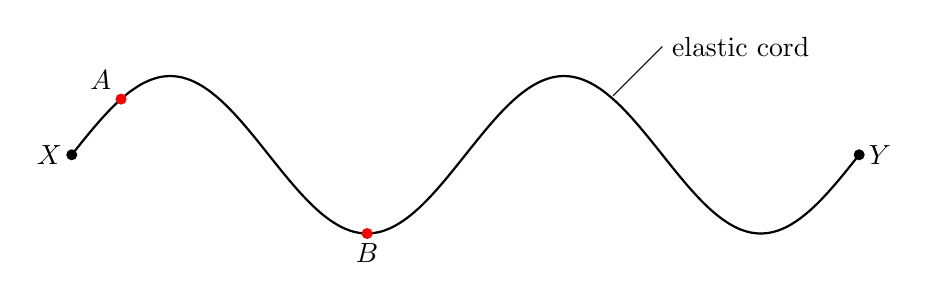
\begin{tikzpicture}[scale=1.25]
	\draw [thick, domain=0:8,samples=80,smooth] plot (\x,{0.8*sin(\x*90)});
	\draw[fill] (0,0) circle (0.05) node[left]{$X$};
	\draw[fill] (8,0) circle (0.05) node[right]{$Y$};
	\draw (5.5, 0.75*0.8) --++ (0.5,0.5) node[right]{elastic cord};
	\draw[fill, red] (0.5, {0.8*sin(45)}) circle(0.05) node[above left, black]{$A$};
	\draw[fill, red] (3, -0.8) circle(0.05) node[below, black]{$B$};
	\end{tikzpicture}
\end{figure}

